In this section the Redux state management solution is used to implement the application.
\subsubsection{Base funtionalities}  \label{par:todo_app_inherited_widget_introduction}
\paragraph{The AppState - }
\label{subpar:todo_app_bloc_core_state}
Redux solution requires the state to be centrilized in a unique location. A model for this centrilized component must be defined to wrap up all the subparts. Subparts of the state have been already modelled in the implementation of the shared parts of the application RIFERIMENTO. They are used now to compose a new class, called AppState, that groups all the subparts in a unique place throughout the entire application. 
\begin{code}
\mbox{}\\
\captionof{listing}{Todo app - Redux - AppState model definition} \mbox{}
		\label{code:2.14}
\begin{minted}{dart}
class AppState {

  VisibilityFilter visibilityFilter;
  List<Todo> todos;
  TabState tabState;

  AppState({this.todos=const [],this.tabState= TabState.todos,this.visibilityFilter= VisibilityFilter.all});
}
\end{minted}
\mbox{}
\end{code}

Notice that the list of filtered todos does not take part in the AppState. In Redux, indeed, the centralized state is kept as simple as possible and the parts of the state that can be computed or derived should be omitted. The filtered list of todo should be computed in the presentation layer when needed. This approach, however, can introduce reduntant computations due to the fact that the filtered list is calculated at every widget build. This is where Selectors come into play; they propose a mechanism based on the memoization techinque in order to reuse precomputed value. This aspect will be deeper investigated later.
\paragraph{The actions - }
\label{subpar:todo_app_bloc_core_state}In order to mutate the state is necessary to define actions. Actions are processed by reducers to produce new states. Actions are just instances of predefined classes. We start defining the action's classes needed to change the state regarding the list of todos. As usual, the first two features to be implemented are the fetching of todos and the setting of the completed field of a specific todo. Due to the way Redux works, asynchronous actions are handled by Middlewares. Reducers, indeed, are pure functions and are not suited for handling asynchronous code. Two actions are defined just for the fetching process. One is called LoadTodoAction and will be intercepted by the middleware which will take care of fetching the todos from the database. The second is called LoadTodoSuccededAction and carries the list of todos fetched from the database. When the fetching process terminates in the middleware a new LoadTodoSuccededAction is emited and handled by reducers in the AppState.
\begin{code}
\mbox{}\\
\captionof{listing}{Todo app - Redux - Loading todos actions definition} \mbox{}
		\label{code:2.14}
\begin{minted}{dart}
class LoadTodoAction{
  @override
  String toString(){
    return "loadTodoAction";
  }
}
class LoadTodoSucceededAction{
  List<Todo> todos;
   LoadTodoSucceededAction(this.todos);
}
\end{minted}
\mbox{}
\end{code}

Another action class is create to handle the setting o the completed field. In this case the action is synchronous and is directly handled by reducers. This new action is called \textit{SetCompletedAction} and contains the id of the todo to be changed and the new value for the completed field.
\begin{code}
\mbox{}\\
\captionof{listing}{Todo app - InheritedWidget - SetCompletedTodoAction definitio} \mbox{}
		\label{code:2.14}
\begin{minted}{dart}
class SetCompletedTodoAction {
  final int id;
  final bool completed;

  SetCompletedTodoAction(this.id, this.completed);
}
\end{minted}
\mbox{}
\end{code}

Two more action are needed to handle the tab and the visibility filter changes. They are called respectively  \textit{SetTabAction} and \textit{SetVisibilityFilterAction}. They contains the new tab value and the new filter value to be set.
\begin{code}
\mbox{}\\
\captionof{listing}{Todo app - Redux - SetTabAction definition} \mbox{}
		\label{code:2.14}
\begin{minted}{dart}
class SetTabAction{
  final TabState newtab;

  SetTabAction(this.newtab);
}

class SetVisibilityFilterAction{
  VisibilityFilter filter;

  SetVisibilityFilterAction(this.filter);
}
\end{minted}
\mbox{}
\end{code}

\paragraph{Reducers - }
\label{subpar:todo_app_bloc_core_state}
Is the turn now for reducer's definition. They will link actions with new states. Even if the usage of the Redux state management solution requires the centralization of the state in a unique component the state’s logic can be in any case be split up in subparts. It is like a tree with a single root where the root is represented by the AppState's reducer.  It can split up in many sub-reducers and every one of them can further split up into other sub-reducers. Therefore the state is segmented and stored in single place, but its pieces can still be managed separately and independently. During the reasoning process is easier to break the whole state into small pieces step by step using a top-down approach, however, in the implementation process, a bottom-up approach is usually used. This is due to the fact that, during the implementation, smaller bricks are required to build bigger components. In this presentation, for example, is not possible to define directly the AppState reducer even if, logically, it should be the first reducer to be implemented. The AppState reducer will be composed by multiple sub reducers, in our case three. There will be a reducer for the list of todos, a reducers for the filter and a reducer for the tab. 
\paragraph{The todoReducer - }
\label{subpar:todo_app_bloc_core_state}
The reducer for the list of todos needs to handle two actions, the LoadTodoSuccedeedAction and the SetCompletedTodoAction. The TodoReducer is tough a combination of two subreducers which handle a specific action. As we already said, reducers are pure functions. They take the previous state and an action and return the next state. The reducer for the LoadTodoSuccedeedAction is called \textit{setLoadedTodo} and just returns the list contained in the received action.
\begin{code}
\mbox{}\\
\captionof{listing}{Todo app - Redux - LoadTodoSuccedeedAction reducer} \mbox{}
		\label{code:2.14}
\begin{minted}{dart}
List<Todo> _setLoadedTodo(List<Todo> todos, LoadTodoSucceededAction action) {
  return action.todos;
}
\end{minted}
\mbox{}
\end{code}
The reducer for the \textit{SetCompletedTodoAction} is called \textit{setCompletedTodo} and takes care of searching in the current todos state the one matching the id contained in the action element. Once the todo is updated the a new instance of the whole list is created and returned. The necessity to create another instance comes from the fact that, in case the state’s list is just updated and not substituted, the transition would not be recognised.
\begin{code}
\mbox{}\\
\captionof{listing}{Todo app - Redux - SetCompletedTodoAction reducer} \mbox{}
		\label{code:2.14}
\begin{minted}{dart}
List<Todo> _setCompletedTodo(List<Todo> todos, SetCompletedTodoAction action) {
  List<Todo> newList= todos.map((todo) => todo.id == action.id
      ? Todo(
          id: action.id,
          name: todo.name,
          description: todo.description,
          completed: action.completed)
      : todo).toList();

  return List.from(newList);
}
\end{minted}
\mbox{}
\end{code}

Now that all the needed reducers has been implemented we  use some tools, the Redux package provides, in order to combine them in a single reducer that binds the received action to the correct sub-reducer. These tools are the \textit{combineReducers} function and the \textit{TypedReducer} class. The \textit{TypedReducer} class is, indeed, a typed class that helps avoiding nested if-else structures which can generate lot of boilerplate and code unreadability. It binds a specific action to a reducer. \textit{combineReducers} , instead, is a function that creates a new reducer composing sub-reducers provided in the form of \textit{TypedReducers}. The two previously defined reducers are now merged into a single one called \textit{todosReducer}.
\begin{code}
\mbox{}\\
\captionof{listing}{Todo app - Redux - combine reducers using combineReducers function} \mbox{}
		\label{code:2.14}
\begin{minted}{dart}
final todoReducer = combineReducers<List<Todo>>([
  TypedReducer<List<Todo>, LoadTodoSucceededAction>(_setLoadedTodo),
  TypedReducer<List<Todo>, SetCompletedTodoAction>(_setCompletedTodo),
]);
\end{minted}
\mbox{}
\end{code}

the alternative would have been to write the \textit{todosReducer} as presented RIERIEMENTO. The output is the same but the code is clearly less readable.
\begin{code}
\mbox{}
\captionof{listing}{Todo app - Redux - combine reducers using the traditional way} \mbox{}
		\label{code:2.14}
\begin{minted}{dart}
final todosReducer = (List<Todo> todos, action) {
  if (action is LoadTodoSucceededAction) {
    return _setLoadedTodo(todos,action);
  } else if (action is SetCompletedTodoAction) {
    return _setCompletedTodo(todos, action);
  } else {
    return state;
  }
};
\end{minted}
\mbox{}
\end{code}

\paragraph{The tab Reducer and the visibility Filter reducer - }
\label{subpar:todo_app_bloc_core_state}
The process is the same as before. Two reducers, called \textit{setTabState} and \textit{setVisibilityFilter}, are created to handle actions of type SetTabAction and SetVisibilityFilter respectively. In both cases the value contained in the action is used to produce a new state. Both of them are used to create other two reducers called \textit{tabReducer} and \textit{visibilityFilterReducer} using the \textit{combineReducers} function introduced earlier. In this case the usage of the \textit{combineReducers} function wasn’t really necessary by the fact that it combines only one reducer. However in case new actions may be introduced it will get handy.
\begin{code}
\mbox{}\\
\captionof{listing}{Todo app - Redux - reducers definition for the tab and the filter state} \mbox{}
		\label{code:2.14}
\begin{minted}{dart}
TabState _setTabState(TabState state, SetTabAction action){
   return action.newtab;
}


VisibilityFilter _setVisibilityFilter(
    VisibilityFilter oldState, SetVisibilityFilterAction action) {
  return action.filter;
}

final tabReducer= combineReducers<TabState>([
  TypedReducer<TabState, SetTabAction>(_setTabState),

]);
final visibilityFilterReducer = combineReducers<VisibilityFilter>([
  TypedReducer<VisibilityFilter, SetVisibilityFilterAction>(
      _setVisibilityFilter)
]);
\end{minted}
\mbox{}
\end{code}

\paragraph{The AppState reducer - }
\label{subpar:todo_app_bloc_core_state}
All the basic bricks have been implemented and can be used now to create the biggest reducer; the AppState reducer. It is a function that takes the current \textit{AppState} and an action. It then composes a new AppState instance using the sub-reducers it is composed of. Every sub-reducer processes the received action in order to understand if it needs to perfom a transition in the part of the state it handles. 
\begin{code}
\mbox{}\\
\captionof{listing}{Todo app - Redux - AppState definition} \mbox{}
		\label{code:2.14}
\begin{minted}{dart}
AppState appStateReducer(AppState appState, action) {
  return AppState(
      todos: todoReducer(appState.todos, action),
      tabState: tabReducer(appState.tabState, action),
      visibilityFilter: visibilityFilterReducer(appState.visibilityFilter,action));
}
\end{minted}
\mbox{}
\end{code}

\paragraph{The Middleware - }
\label{subpar:todo_app_bloc_core_state}
All the necessary to start accessing the state in the presentation layer is settled up but the way in which the todos are fetched from the database is not clear yet. Two actions were set up for this purpose but only one has been handled by a reducer. The process of fetching todos from the database is not immediate. It is asynchronous with respect to the application workflow. Reducers are not suited for handling asynchronous code, they need to be pure and as simple as possible. There are many ways, in practice, to deal with asynchronous code using Redux  but, the most correct one (and also the one proposed in the documentation) is to use Middlewares. Middlewares has been introduce HERE RIEFERIMENTO. They act as a sort of proxy between actions dispatch and reducers. One or more middlewares can be set to execute on actions call. They are used to handle asynchronous code but also action that generate side effects. In our case, an action of type LoadTodoAction has been defined but is not handled by any reducer yet and is ignored once received. However, if dispatched, it will pass through one or more middleware before reaching the reducers. Is necessary tough to set up a middleware that intercepts it and starts the fetching process. A middleware is just a function that takes three parameters: the store, an action and the next dispatcher. It processes the action , probably accessing the store, and then pass the action to the next middleware. A new middleware function is defined and called \textit{loadTodoMiddleware}. It  checks if the dispatched action if of type LoadTodoAction and, in case it is, starts to load the todos from the database. Once the fetching process is completed it dispatches an action of type LoadTodoSuccededAction that contains the list of fetched todo. We previously set up a specific reducer in order to handle this type of action in the AppState reducer.
\begin{code}
\mbox{}\\
\captionof{listing}{Todo app - Redux - loadTodosMiddleware middleware definition} \mbox{}
		\label{code:2.14}
\begin{minted}{dart}
void loadTodosMiddleware(Store<AppState> store, action, NextDispatcher next) {

  if (action is LoadTodoAction) {
    TodoRepository.loadTodos().then((todos) {store.dispatch(LoadTodoSucceededAction(todos));} );
  }
  next(action);
}
\end{minted}
\mbox{}
\end{code}

All the ingredients are now available to start composing our UI.

\paragraph{Making the state accessible - }
\label{subpar:todo_app_bloc_core_state}
Redux uses Provider widgets to make the state accessible down the widgets tree. The state is unique and tough should  be placed in the root of the widgets tree or some part of the tree would not be covered by its accessibility. To do so, a StoreProvider widget is positioned at the root of app, right below the MyApp widget. An object of type Store must be provided to the StoreProvider widget, in the \textit{store }field. The typed class Store is provided by the redux package. In our case the global state is of the type AppState defined above. The Store class constructor takes three parameters. The reducer for the AppState , an instance of type AppState that identifies the initial state and a list of middlewares. In our case a single middleware is passed. In order to fetch the todos at the application start we will use the \textit{init} method of stateful widgets.  The HomePage is already stateful and its \textit{init} method is used in order to dispatch the first action : the LoadTodosAction. For simplicity the function to be executed in the init method is passed from the MyApp widget, where the store is already available, to the HomePage using a newly created parameter.
\begin{code}
\mbox{}\\
\captionof{listing}{Todo a
pp - Redux - Widgets tree root definition} \mbox{}
		\label{code:2.14}
\begin{minted}{dart}
void main() {
  WidgetsFlutterBinding.ensureInitialized();
  runApp(MyApp(
      store: Store<AppState>(appStateReducer,
          initialState: AppState(), middleware: [loadTodosMiddleware])));
}

class MyApp extends StatelessWidget {
  final Store<AppState> store;

  const MyApp({Key? key, required this.store}) : super(key: key);

  @override
  Widget build(BuildContext context) {
    print("Building Material App");
    return StoreProvider(
      store: store,
      child: MaterialApp(initialRoute: "/",
        routes: {
          "/": (context) => HomePage(onInit: (){
            store.dispatch(LoadTodoAction());
            },),
            (...)
         },
      ),
    );

  }
}
\end{minted}
\mbox{}
\end{code}

Inside the HomePage, the \textit{initState} method is set up in order to dispatch a LoadTodoAction using the function passed as parameter by the MaterialApp widget. In order to access the store, a StoreConnector widget is used. A StoreConnector widget takes two functions in its \textit{converter }and \textit{builder }fields. The \textit{converter} function takes the state and creates a viewmodel containing the minimal information necessary to build the widget. The \textit{builder} function actually uses the viewmodel in order to create the widget. The viewmodel is really important because idenfies the prospective from which, the widget, is looking at the centralized state. If the viewmodel changes the widget is rebuilt. Not always a state change produces a viewmodel change. The StoreConnector widget is a typed widget also and takes two types in its definition/usage: the store's type, the AppState, and the viewmodel's type, in our case just a TabState object. The HomePage, indeed, only needs the part of the state related to the tab and, for this reason, it is not necessary to create an ad hoc viewmodel. The model of the TabState defined hereRIFERIMENTO is enough to contain the interesting part of the state. In the \textit{converter }field a function is provided which manipulates the state returning the current TabState value. The \textit{builder} field is populated with a function that returns a Scaffold widget. Inside this function, the current context and the object returned from the converter function can be used. This last one is used to populate the Scaffold widget as usual.
\begin{code}
\mbox{}\\
\captionof{listing}{Todo app - Redux - state integration in the HomePage} \mbox{}
		\label{code:2.14}
\begin{minted}{dart}
@override
void initState() {
  widget.onInit();
  super.initState();
}

@override
Widget build(BuildContext context) {
  print("Building HomePage");

  return StoreConnector<AppState, TabState>(
    converter: (store) => store.state.tabState,
    builder: (context, currTab) {
      return Scaffold(
          appBar: AppBar(...),
          body: currTab == TabState.todos ? const TodoView() : const Stats(),
          bottomNavigationBar: const TabSelector(),
          floatingActionButton: currTab == TabState.todos
              ? FloatingActionButton(...)
              : Container());
    },
  );
}
\end{minted}
\mbox{}
\end{code}

We can now start implementing the component widgets using the AppState but, first, a short digression about Selectors is taken.
\paragraph{Selectors - }
\label{subpar:todo_app_bloc_core_state}
They are introduced hereRIFERIMENTO . Selectors are used to compute those parts of the state that entirely depends on other parts. In our case, for example, the filtered list is not included in the AppState with the idea of computing it in the presentation layer. This decision also comes from the fact that would be hard to syncornize it with the changes in the todos list and in the filter if situated in the centralized state. The easiest way to deal with the filtered list is to compute it in the UI layer before building the TodoView widget. However, this way of doing can become quite heavy soon by the fact that the computation of the filtered list is perfomed every time the widget is rebuilt. In this scenario Selectors come into play to memoize the previously computed value and to reuse them once accessed. Selectors are just functions that take as input the state an return an element composed with it. All the memorization part is perfomed by a third party package called \textit{Reselect}. In order to use this package it must be included in the pubspec.yaml file under the \textit{dependencies} field. It provides some functions with the called \textit{createSelector} that take care of memoizing some values and understanding when to recompute them. Selectors can be simple o composed. For example, two simple selectors can be implemented in our case. One  takes the state and return the filter and the other takes the state and returns the list of todos.
\begin{code}
\mbox{}\\
\captionof{listing}{Todo app - Redux - base Selectors definition} \mbox{}
		\label{code:2.14}
\begin{minted}{dart}
final todosSelector = (AppState state) => state.todos;

final filterSelector = (AppState state) => state.visibilityFilter;
\end{minted}
\mbox{}
\end{code}

Selectors can be composed with other selector to create articulated objects. Selectors are composed using the \textit{createSelector} function followed by a number. For example, a selector computing the list of completed todos can be built using the \textit{todosSelector }and the \textit{createSelector1} function. The same con be done to compute the list of pending todos. Another Selector is created to finally compute the filtered list. It uses the four other selectors we just implemented and the \textit{createSelector4 }function. Besides of making the code more readable , selectors, allow to optimize the application's performances.
\begin{code}
\mbox{}\\
\captionof{listing}{Todo app - Redux - composed  Selectors definition} \mbox{}
		\label{code:2.14}
\begin{minted}{dart}
final todosSelector = (AppState state) => state.todos;

final filterSelector = (AppState state) => state.visibilityFilter;

final completedTodosSelector = createSelector1(
    todosSelector,
    (List<Todo> todos) =>
        todos.where((todo) => todo.completed == true).toList());

final pendingTodosSelector = createSelector1(
    todosSelector,
    (List<Todo> todos) =>
        todos.where((todo) => todo.completed == false).toList());

final filteredTodosSelector = createSelector4(
    todosSelector, filterSelector, completedTodosSelector, pendingTodosSelector,
    (List<Todo> todos, VisibilityFilter filter, List<Todo> completed,
        List<Todo> pending) {
  switch (filter) {
    case VisibilityFilter.completed:
      return completed;
    case VisibilityFilter.notCompleted:
      return pending;
    case VisibilityFilter.all:
      return todos;
  }
});
\end{minted}
\mbox{}
\end{code}

\paragraph{The TodoView component - }
\label{subpar:todo_app_bloc_core_state}
After this short digression about selectors, we are ready to set up the TodoView component. The ListView widget is wrapped into a StoreConnector widget typed with the AppState and List<Todo> types. The TodoView component just needs to access the part of the state concerning the filtered list of todos that is representable with an object of type List<Todo>. The list of filtered todos is not directly available in the AppState but selectors can be used to compute it. In the \textit{converter }field of the StoreConnector widget, a function is provided which takes the store and returns the filtered list using the \textit{filteredTodosSelector}. The \textit{converter} function output is available inside the \textit{builder} field's function and is used to populate the ListView widget as usual. 
\begin{code}
\mbox{}\\
\captionof{listing}{Todo app - Redux - state integration in the TodoView component} \mbox{}
		\label{code:2.14}
\begin{minted}{dart}
class TodoView extends StatelessWidget {
  const TodoView({Key? key}) : super(key: key);

  @override
  Widget build(BuildContext context) {
    return StoreConnector<AppState, List<Todo> >(
        builder: (context, todos) {
          print("Building TodoView");
          return ListView.builder(
            itemCount: todos.length,
            itemBuilder: (context, index) {
              return TodoItem(
                todo: todos.elementAt(index),
              );
            },
          );
        },
        converter: (store) {
          return filteredTodosSelector(store.state);
        });
  }
}
\end{minted}
\mbox{}
\end{code}

\paragraph{The TodoItem component - }
\label{subpar:todo_app_bloc_core_state}

The TodoItem component does not require any modification with respect to the implementation proposed HERE RIFERIMENTO. It just receives a todo from the parent widget and exposes it to the user. The only missing part is the \textit{onChanged} field of the Checkbox widget which is still to be implemented. Inside the \textit{onChage} field, a function must be provided which updates the \textit{completed} field of the visualized todo. The store is accessed using the \textit{of} method of the StoreProvider widget (the of method gets the nearest instance of provided type, in our case AppState). The store is then used to dispatch an action of type SetCompletedTodoAction created using the id, of the visualized todo, and the \textit{completed} Boolean value provided by the \textit{onChange} fuction.

\begin{code}
\mbox{}
\captionof{listing}{Todo app - Redux - state integration in the TodoItem component} \mbox{}
		\label{code:2.14}
\begin{minted}{dart}
Checkbox(
    value: todo.completed,
    onChanged: (completed) {
      StoreProvider.of<AppState>(context).dispatch(
          SetCompletedTodoAction(todo.id, completed!));
    }),
\end{minted}
\mbox{}
\end{code}

\paragraph{The VisibilityFilterSelector component - }
\label{subpar:todo_app_bloc_core_state}
The VisibilityFilterSelector component only accesses the part of the state concerning the filter. The entire DropdownButton widget is wrapped into a StoreConnector widget. The StoreConnector’s \textit{converter} field  is filled with a function taking the store and returning the current filter value. To do so, it uses the \textit{filterSelector} implemented earlier. The output of the \textit{converter} function is accessed in the \textit{builder} field function and used to populate the DropdownButton widget. The function used in the \textit{onChanged} field of the DropdownMenuItem widgets gets an instance of the store using the StoreProvider widget’s \textit{of} method and dispatches an action of type SetVisibilityFilterAction using the DropdownMenuItem 's filter value.
\begin{code}
\mbox{}\\
\captionof{listing}{Todo app - Redux - state integration in the VisibilityFilterSelector component} \mbox{}
		\label{code:2.14}
\begin{minted}{dart}
@override
Widget build(BuildContext context) {
  return StoreConnector<AppState, VisibilityFilter>(
    converter: (store) => filterSelector(store.state),
    builder: (context, activeFilter) {
      print("Building Visibility filter");

      return DropdownButton<VisibilityFilter>(
        value: activeFilter,
        items: (...),
        onChanged: (filter) {
          StoreProvider.of<AppState>(context)
              .dispatch(SetVisibilityFilterAction(filter!));
        },
      );
    },
  );
\end{minted}
\mbox{}
\end{code}

\paragraph{The TabSelector component - }
\label{subpar:todo_app_bloc_core_state}
Also in this case, the TabSelector component requires to read and write the AppState. A StoreConnector widget is used to wrap the BottomNavigationBar widget and to connect it to the state. The viewmodel to be returned by the \textit{converter} function is just an object of type TabState. An arrow function returning the current AppState’s tab value is provided to the converter field. The function output is then used in the \textit{builder} field's function to populate the BottomNavigationBar widget. The \textit{onTap} field of the BottomNavigatioBar widget is filled with a function that dispatches an action of type SetTabAction when fired.
\begin{code}
\mbox{}\\
\captionof{listing}{Todo app - Redux - state integration into TabSelector component} \mbox{}
		\label{code:2.14}
\begin{minted}{dart}
class TabSelector extends StatelessWidget {
  const TabSelector({Key? key}) : super(key: key);

  @override
  Widget build(BuildContext context) {

    return StoreConnector<AppState, TabState>(
      converter:(store)=>store.state.tabState,
      builder: (context, currTab) {
        print("Building Tab Selector");

        return BottomNavigationBar(
          currentIndex: TabState.values.indexOf(currTab),
          onTap: (index)=>StoreProvider.of<AppState>(context).dispatch(SetTabAction(TabState.values.elementAt(index))),
          items: (...)
        );
      },
    );
  }
}
\end{minted}
\mbox{}
\end{code}

\paragraph{The Stats component - }
\label{subpar:todo_app_bloc_core_state}
The stats component only requires to read the state. The Center widget is wrapped into a StoreConnector widget. In the \textit{converter} field's function the \textit{completedTodoSelector} selector is used to access the list of completed todos. In this case the viewmodel to be outputted is just an int value representing the number of completed todos.
\begin{code}
\mbox{}\\
\captionof{listing}{Todo app - Redux - state integration into Stats component} \mbox{}
		\label{code:2.14}
\begin{minted}{dart}
class Stats extends StatelessWidget {
  const Stats({Key? key}) : super(key: key);

  @override
  Widget build(BuildContext context) {
    return StoreConnector<AppState, int>(
      builder: (context, completed) {
        print("Building Stats");
        return Center(child: Text(completed.toString()));
      },
      converter: (store) {
        return completedTodosSelector(store.state).length;
      },
    );
  }
}
\end{minted}
\mbox{}
\end{code}

At this point all the base functionalities have been implemented and are working fine.
 

\subsubsection{Features addition}  \label{par:todo_app_inherited_widget_introduction}

The first thing to do is to make the state provide a way of adding and updating todos. For this purpose two new actions are created with the name AddTodoAction and UpdateTodoAction respectively. In the AddTodoAction, are contained the name and the description for the todo to be create. In the UpdateTodoAction, besides the new name and description, also the id of the todo to be modified is contained.
\begin{code}
\mbox{}\\
\captionof{listing}{Todo app - Redux - AddTodoAction and UpdateTodoAction definition} \mbox{}
		\label{code:2.14}
\begin{minted}{dart}
class AddTodoAction {
  final String name;
  final String desc;

  AddTodoAction(this.name, this.desc);
}

class UpdateTodoAction{
  final String name;
  final String desc;
  final int id;

  UpdateTodoAction(this.name,this.desc,this.id);
}
\end{minted}
\mbox{}
\end{code}

In order to handle these new actions two new reducers must be created. They are called respectively \textit{addTodo} and \textit{updateTodo}. The \textit{addTodo} reducer first creates a new todo using the information contained in the \textit{AddTodoAction}  instace and a newly generated unique id. Then, it creates a new list instace and populates it with the elements of the old list plus the new todo.
\begin{code}
\mbox{}\\
\captionof{listing}{Todo app - Redux - AddTodoAction's reducer definition} \mbox{}
		\label{code:2.14}
\begin{minted}{dart}
List<Todo> _addTodo(List<Todo> todos, AddTodoAction action) {
  Random rand = Random();
  List<int> ids = todos.map((todo) => todo.id).toList();
  int newId = rand.nextInt(1000) + 2;
  while (ids.contains(newId)) {
    newId = rand.nextInt(1000) + 2;
  }
  Todo newTodo = Todo(
      id: newId,
      name: action.name,
      description: action.desc + " " + newId.toString(),
      completed: false);

  return List.from(todos)..add(newTodo);
}
\end{minted}
\mbox{}
\end{code}

The \textit{updateTodo} reducer first modifies the todo with the id matching the one contained in the action. Then, it generates a new list and fills it with the element contained in the current one.
\begin{code}
\mbox{}\\
\captionof{listing}{Todo app - Redux - UpdateTodoAction's reducer definition} \mbox{}
		\label{code:2.14}
\begin{minted}{dart}
List<Todo> _updateTodo(List<Todo> todos, UpdateTodoAction action){

  List<Todo> newList= todos.map((todo) => todo.id == action.id
      ? Todo(
      id: action.id,
      name: action.name,
      description: action.desc,
      completed: todo.completed)
      : todo).toList();

  return List.from(newList);
}
\end{minted}
\mbox{}
\end{code}

These new reducers are then combined with the already existing ones in the \textit{combineReducers} function and linked with the corresponding action using the typed class \textit{TypedReducer}.
\begin{code}
\mbox{}\\
\captionof{listing}{Todo app - Redux - combining new reducers to the old ones} \mbox{}
		\label{code:2.14}
\begin{minted}{dart}
final todoReducer = combineReducers<List<Todo>>([
  TypedReducer<List<Todo>, AddTodoAction>(_addTodo),
  TypedReducer<List<Todo>, LoadTodoSucceededAction>(_setLoadedTodo),
  TypedReducer<List<Todo>, SetCompletedTodoAction>(_setCompletedTodo),
  TypedReducer<List<Todo>, UpdateTodoAction>(_updateTodo),
]);
\end{minted}
\mbox{}
\end{code}

The AppState can now handle actions of type AddTodoAction and UpdateTodoAction. These new functionalities can now be used in the AddTodoPage and in the UpdateTodoPage. The StoreProvider widget has been positioned in the root of the application to be available in all the subtrees. Is sufficient, tough, to access the store in the AddTodoPage and dispatch an action of type AddTodoAction, when the TextButton widget is tapped.
\begin{code}
\mbox{}\\
\captionof{listing}{Todo app - Redux - using the AddTodoAction in the AddTodoPage} \mbox{}
		\label{code:2.14}
\begin{minted}{dart}
TextButton(
    onPressed: () {
      final AddTodoAction action= AddTodoAction(textControllerName.text, textControllerDesc.text);
      StoreProvider.of<AppState>(context).dispatch(action);
      Navigator.pop(context);
    },
    child: const Text("Create"))
\end{minted}
\mbox{}
\end{code}

The same is done in the UpdateTodoPage. Once the TextButton widget is tapped an action of type UpdateTodoAction is dispatched.
\begin{code}
\mbox{}\\
\captionof{listing}{Todo app - Redux - using the UpdateTodoAction into the UpdateTodoPage} \mbox{}
		\label{code:2.14}
\begin{minted}{dart}
TextButton(
    onPressed: () {
      final UpdateTodoAction action= UpdateTodoAction(textControllerName.text,textControllerDesc.text,widget.todo.id);
      StoreProvider.of<AppState>(context).dispatch(action);
      Navigator.pop(context);
    },
    child: const Text("Confirm"))
\end{minted}
\mbox{}
\end{code}

All the features have been successfully added.
\subsubsection{Rendering optimization}  \label{par:todo_app_inherited_widget_introduction}

In order to perform the optimizations we will leverage on the fact that the StoreConnector widgets only rebuilds when the viewmodel, it relies on, changes. Or better, this happens when a specific field of the StoreConnector widget, called \textit{distinct}, is set to true. This feature, the Redux package provides, makes the optimization process really easy. We just need to define the correct viewmodel and provide it with the correct equality operator. Some changes must be done in the TodoView widget and in the TodoItem widget. Firstly, the TodoItem widget needs to interact with the state in order to understand when a change regarding its todo is performed. For the moment , indeed, the TodoItem widget just receives a todo instance from the parent widget and exposes it to the user.A StoreConnector widget is used to read the state in the TodoItem widget. The complete instance of the todo to be visualized is not necessary anymore but the id only is enough. Using the id , the corresponding todo is searched in the store by the \textit{converter} field’s function and passed to the \textit{builder} field. The widget returned by the \textit{builder} function remains the same with the only exception that it uses the todo instance got from the store instead of the one passed by the parent widget. 
\begin{code}
\mbox{}\\
\captionof{listing}{Todo app - Redux - make the TodoItem component read the state} \mbox{}
		\label{code:2.14}
\begin{minted}{dart}
class TodoItem extends StatelessWidget {
  final int id;

  const TodoItem({Key? key, required this.id})
      : super(key: key);

  @override
  Widget build(BuildContext context) {
    return StoreConnector<AppState, Todo>(
      distinct: true,
        converter: (store) =>
            store.state.todos.firstWhere((element) => element.id == id),
        builder: (context, todo) {
          print("building: Todo Item \$id ");

          return InkWell(. . .);
        });
  }
}
\end{minted}
\mbox{}
\end{code}

Now that the TodoItem widget listens for its own todo changes, the optimization process concerning the TodoItem widget is automatically performed. We said, indeed, that the StoreConnector widget is rebuilt every time its viewmodel changes and we set the viewmodel as the corresponding todo instance in the AppStore. Once a state change occurs, the StoreConnector widget compares the current todo with the new one and, in case they differ, it rebuilds. To notice that this mechanism works because we redefined the equality operator between objects of type Todo HERE RIFERIMENTO. An object of type Todo is equal to another one if all their internal values match. This equality differs from the traditional one by the fact that do not check for the entity’s equality. Indeed, if it would, the two todos would appear to be different everytime. This because, once a new state is emitted, the list of todos is recreated from scratch and its internal todos are replaced with new instances. In the dart language two different objects end to be different also if their internal values are exactly the same. This way of handling object already showed up numerous times in this overview and will show up even more in the next implementations. Going back to the to the TodoItem component , it already uses the correct equality operator to compare different viewmodels and so is capable to understand when to rebuild autonomously. The same process must be done in the TodoView widget. It already uses a StoreConnector widget to derive the list of filtered todos from the store. However, as we just said, two different plain lists appear to be always different by default also if their internal aspects matches. Moreover, it is not possible to redefine the equality operator for lists and, in case, it would not be a good idea. A simple way to handle this scenario is to create an ad hoc viewmodel and redefine its equality operator in order to match our own rebuilding logic. To do so, a local class is created and called ViewModel. This local class just contains a list of todos.
\begin{code}
\mbox{}\\
\captionof{listing}{Todo app - Redux - TodoView ad hoc ViewModel definition} \mbox{}
		\label{code:2.14}
\begin{minted}{dart}
class _ViewModel {
  final List<Todo> todos;

  _ViewModel({required this.todos});

}
\end{minted}
\mbox{}
\end{code}

 Inside the ViewModel class the equality operator is overridden making two ViewModel instances equal when their length matches and their internal ids match too. In this way the TodoView widget is rebuild only in case the filtered todos list has reported a structural change. (structural and not structural changes are exaplained HERE RIFERIMENTO). 
\begin{code}
\mbox{}\\
\captionof{listing}{Todo app - Redux - ViewModel equality operator override} \mbox{}
		\label{code:2.14}
\begin{minted}{dart}
  @override
  bool operator ==(Object other) {
    return ((other is _ViewModel) &&
        todos.length == other.todos.length &&
        todos.every(
            (todo) => other.todos.any((element) => todo.id  == element.id)));
  }

  @override
  // TODO: implement hashCode
  int get hashCode => todos.hashCode;
\end{minted}
\mbox{}
\end{code}

After setting the \textit{distinct} field to true and modifying the \textit{converter} function to return a ViewModel instead of a plain List the optimizations are basically done.
\begin{code}
\mbox{}\\
\captionof{listing}{Todo app - Redux - TodoView renders optimization} \mbox{}
		\label{code:2.14}
\begin{minted}{dart}
class TodoView extends StatelessWidget {
  const TodoView({Key? key}) : super(key: key);

  @override
  Widget build(BuildContext context) {
    return StoreConnector<AppState, _ViewModel>(
        distinct: true,
        builder: (context, vm) {
          print("Building TodoView");
          return ListView.builder(
            itemCount: vm.todos.length,
            itemBuilder: (context, index) {
              return TodoItem(
                id: vm.todos.elementAt(index).id,
              );
            },
          );
        },
        converter: (store) {
          return _ViewModel(todos: filteredTodosSelector(store.state));
        });
  }
}
\end{minted}
\mbox{}
\end{code}

To put the  the icing on the cake we set the \textit{distinct} field to true also in the VisibilityFilterSelector component and in the TabSelector component. In this way they are rebuilt only in case their prospective of the state changes and not at every state transition.

\subsubsection{Conclusions} \mbox{} \\
\label{subpar:render_optimizations_inherited_widget}
\begin{table}[H]
    \caption*{\textbf{Recap}}
    \centering 
    
    \begin{tabular}{| l | c | c | c |}
    \hline
    \rowcolor{bluepoli!40} % comment this line to remove the color
    \hline
     & \textbf{lines of code} & \textbf{time} & \textbf{classes} \T\B \\
    \hline
    \textbf{base functionalities} & 156 & 9-11 h & 6 \T\B \\ 
    \textbf{feature addition} & 50 & 15-20 m & 2 \T\B\\ 
    \textbf{rendering optimization} & 28 & 1 h & 1
    \T\B\\
    \hline
    \end{tabular}
    \\[10pt]
    \caption{Caption of the Table to appear in the List of Tables.}
    \label{table:example}
\end{table}

\begin{figure}[H]
 \caption*{\textbf{Hours}}
\centering
\begin{tikzpicture}

\pie[rotate = 60]{
    88.2/Base functionalities ,
    3/Feature addition,
    8.8/Optimizations 
    }

\end{tikzpicture}
 \caption{Caption of the Table to appear in the List of Tables.}
\end{figure}
\begin{figure}[H]

\caption*{\textbf{Lines}}
\centering
\begin{tikzpicture}

\pie[rotate =90]{57.3/Structure - 314,
    29.5/Base functionalities - 367,
    9.12/Feature addition - 67,
    5.11/Optimizations - 33
    }
 
\end{tikzpicture}
 \caption{Caption of the Table to appear in the List of Tables.}
\end{figure}



\begin{figure}[H]
    \centering
    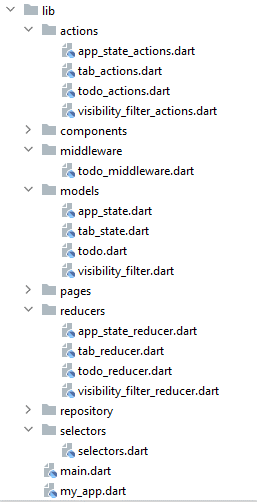
\includegraphics[width=0.6\textwidth]{Images/struttura_cartelle_redux.png}
    \caption{Show the tree structure after the FloatingActionButton in the HomePage is tapped.}
    \label{fig:add_todo_page_tree_structure}
\end{figure}
Down below some images taken from an execution of the application. In this execution ,six todos are randomly created and only two of them are marked as completed. 

\begin{figure}[H]
    \centering
    \subfloat[todos tab runtime UI.\label{fig:todos_tab_UI}]{
        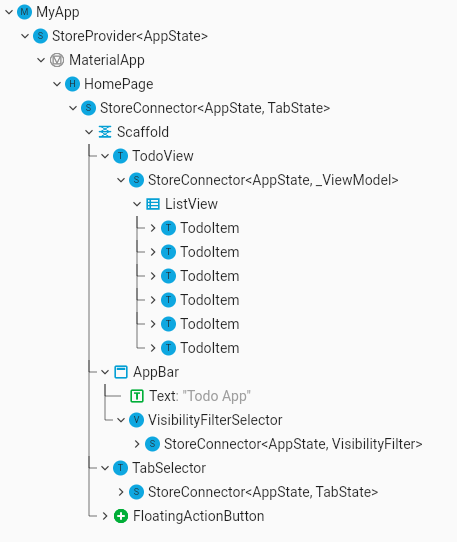
\includegraphics[scale=0.6]{Images/albero_redux_todos.png}
    }
    \quad
    \subfloat[todos tab runtime widget tree.\label{fig:todos_tab_tree}]{
        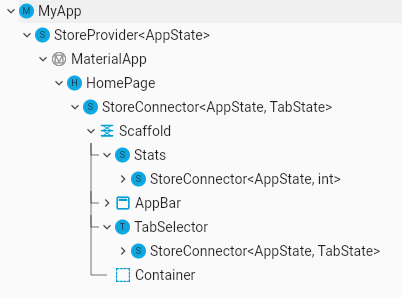
\includegraphics[scale=0.6]{Images/albero_redux_stats.png}
    }
    \caption{Show the runtime Widget's tree and UI when visualizing todos tab.}
    \label{fig:todos_tab}
\end{figure}


Figure~\ref{fig:todos_tab_UI} shows how the application's UI looks like after few seconds from the start. Figure~\ref{fig:todos_tab_tree} show the widget's tree related with the run. Notice the TodoInheritedData widget as a child of the HomePage widget,it provides the state to the subtree.
